\vspace{0.2in}\noindent{\textbf{\underline{ニュースアンカーとして検出した発話の時間による評価}}}\par
k-meansによるニュースアンカーの発話の個数による発話検出精度を図\ref{fig:result_anchor_kmeans_time}、$Th_{time}$を変更してニュースアンカーの発話の時間による発話検出精度が最も高いF-measureを示した条件の結果を図\ref{table:baseline_time} $\sim$ 図\ref{fig:result_anchor_prob3_time}に示す。その他の条件の結果は付録\ref{other_result_time}で記載する。また、図\ref{baseline_kmeans_fmeasure_time} $\sim$ 図\ref{prob3_fmeasure_time}に示された結果の中で、最も高いF-measureをとったときの各ニュース番組のニュースアンカーの発話検出精度とニュースアンカーとして検出したクラスタ数を表\ref{table:baseline_eachnews_time} $\sim$ 表\ref{table:prob3_eachnews_time}に示す。

\begin{figure}[H]
  \centering
    \begin{tabular}{c}
 
%----- recall -----
 
      \begin{minipage}{0.40\hsize}
        \centering
          \subfigure[Recall]{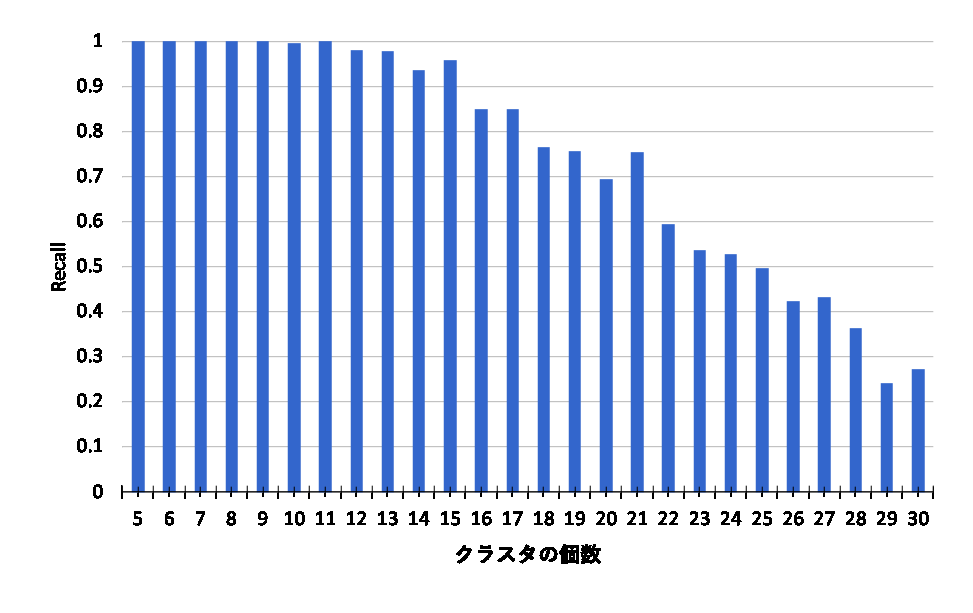
\includegraphics[keepaspectratio, scale=0.45]
                          {./time/figure/result_time_r.eps}}
      \end{minipage}

      \begin{minipage}{0.06\hsize}
        \hspace{0.5mm}
      \end{minipage}
 
%----- precision -----
 
      \begin{minipage}{0.40\hsize}
        \centering
          \subfigure[Precision]{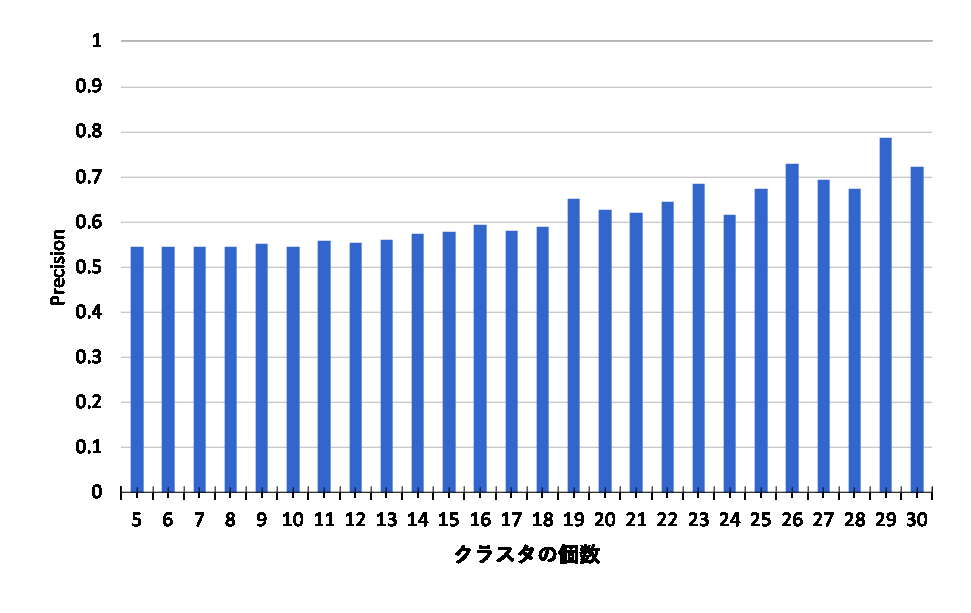
\includegraphics[keepaspectratio, scale=0.45]
                          {./time/figure/result_time_p.eps}}
      \end{minipage} \\

      \begin{minipage}{0.06\hsize}
        \vspace{5mm}
      \end{minipage} \\
 
 
%----- fmeasure -----
 
      \begin{minipage}{0.40\hsize}
        \centering
          \subfigure[F-measure]{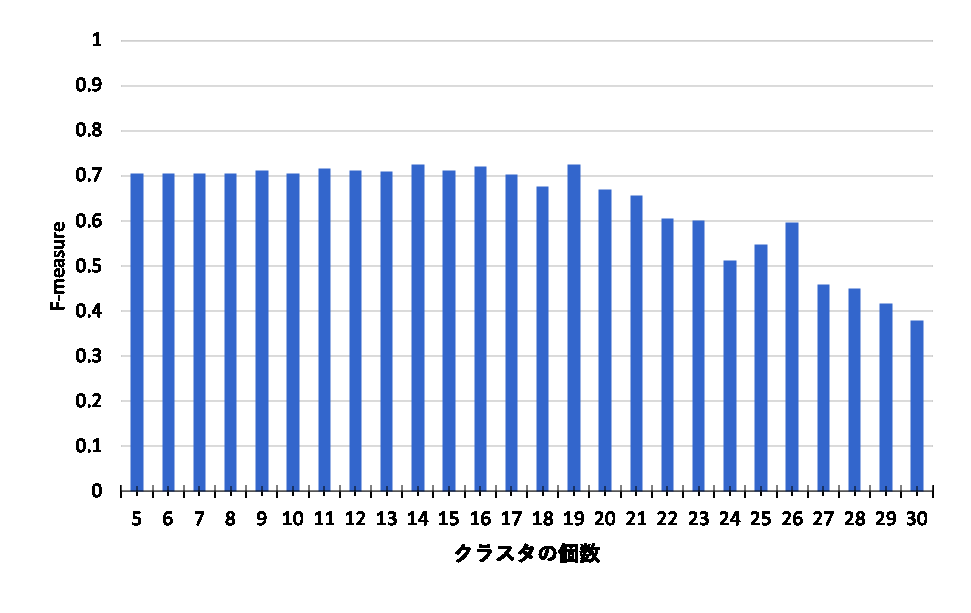
\includegraphics[keepaspectratio, scale=0.45]
                          {./time/figure/result_time_f.eps} \label{baseline_kmeans_fmeasure_time}}
      \end{minipage}

      \begin{minipage}{0.06\hsize}
        \hspace{0.5mm}
      \end{minipage}


    \end{tabular}
\caption{Baseline1による発話区間検出精度 \label{fig:result_anchor_kmeans_time}}
\end{figure} 


\begin{table}[H]
  \begin{center}
    \caption{Baseline1による各ニュース番組音声のニュースアンカーの発話検出精度(クラスタの個数=12) \label{table:baseline_eachnews_time}}
    \begin{tabular}{|c||c|c|c|c|} \hline
データID & Recall & Precision & F-meature & 作成したクラスタ数\\ \hline
ニュース1 & 0.818 & 0.634 & 0.714 & 7\\ \hline
ニュース2 & 0.915 & 0.376 & 0.533 & 10\\ \hline
ニュース3 & 0.966 & 0.537 & 0.690 & 11\\ \hline
ニュース4 & 0.776 & 0.545 & 0.640 & 11\\ \hline
ニュース5 & 0.829 & 0.680 & 0.747 & 11\\ \hline
計 & 0.981 & 0.575 & 0.725 & - \\ \hline
    \end{tabular}
  \end{center}
\end{table}


\begin{figure}[H]
  \centering
    \begin{tabular}{c}
 
%----- recall -----
 
      \begin{minipage}{0.40\hsize}
        \centering
          \subfigure[Recall]{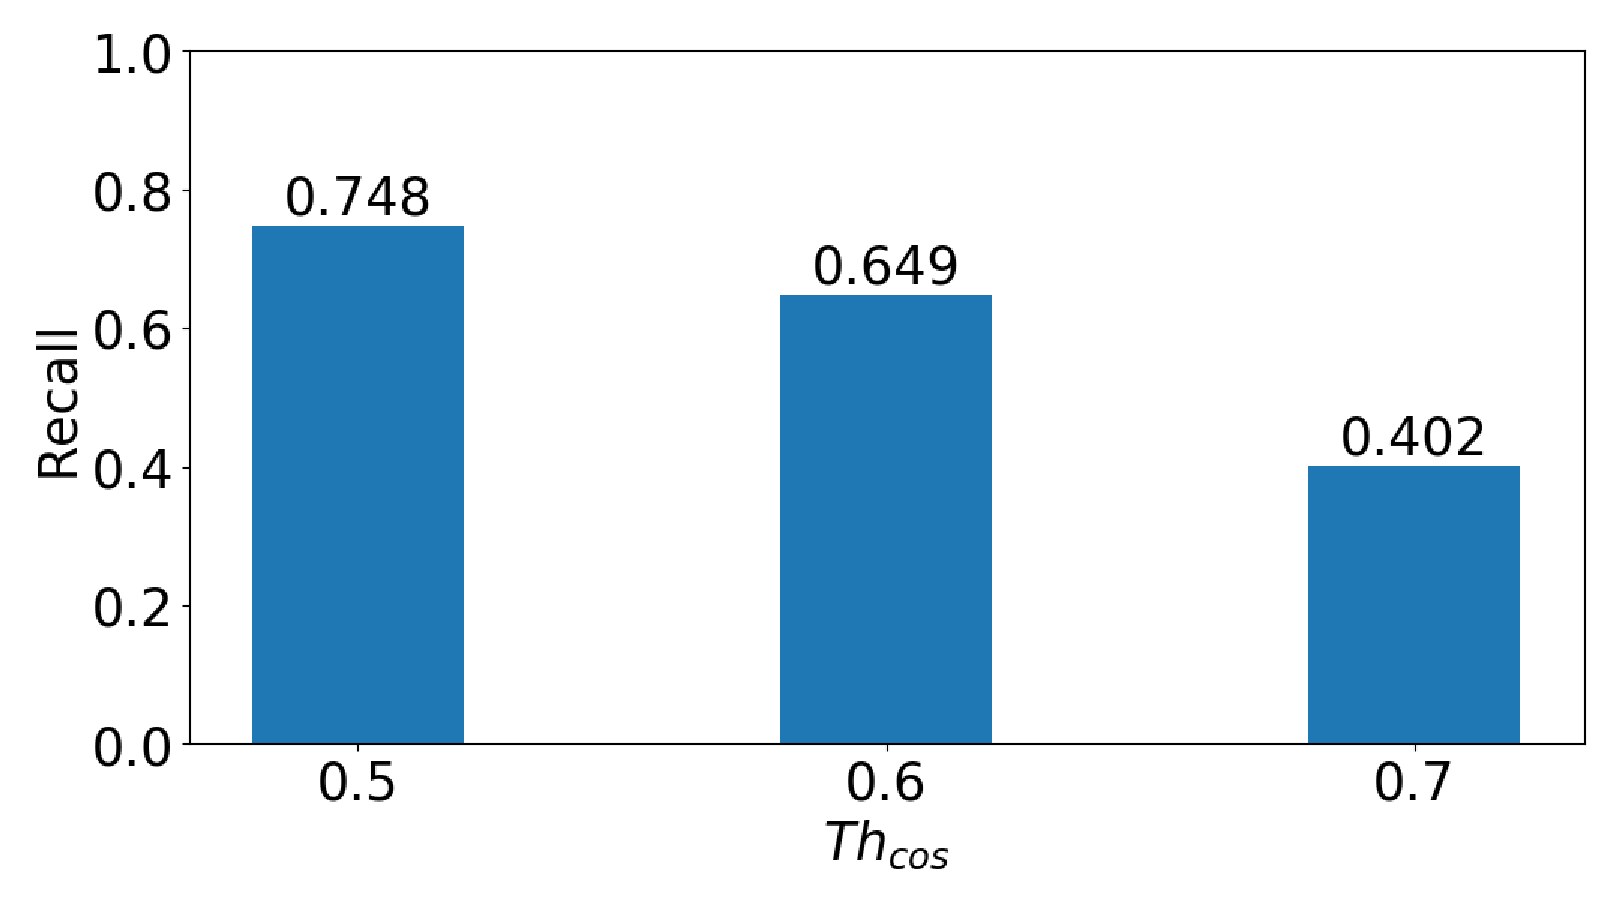
\includegraphics[keepaspectratio, scale=0.25]
                          {./time/figure/baseline_r.eps}}
      \end{minipage}

      \begin{minipage}{0.06\hsize}
        \hspace{0.5mm}
      \end{minipage}
 
%----- precision -----
 
      \begin{minipage}{0.40\hsize}
        \centering
          \subfigure[Precision]{\includegraphics[keepaspectratio, scale=0.25]
                          {./time/figure/baseline_p.eps}}
      \end{minipage} \\

      \begin{minipage}{0.06\hsize}
        \vspace{5mm}
      \end{minipage} \\
 
 
%----- fmeasure -----
 
      \begin{minipage}{0.40\hsize}
        \centering
          \subfigure[F-measure]{\includegraphics[keepaspectratio, scale=0.25]
                          {./time/figure/baseline_f.eps} \label{baseline_fmeasure_time}}
      \end{minipage}

      \begin{minipage}{0.06\hsize}
        \hspace{0.5mm}
      \end{minipage}


    \end{tabular}
\caption{Baseline2による発話区間検出精度 \label{table:baseline_time}}
\end{figure} 


\begin{table}[H]
  \begin{center}
    \caption{Baseline2による各ニュース番組音声のニュースアンカーの発話検出精度($Th_{cos}=0.5$) }
    \begin{tabular}{|c||c|c|c|c|} \hline
データID & Recall & Precision & F-meature & 作成したクラスタ数\\ \hline
ニュース1 & 0.992 & 0.705 & 0.824 & 1 \\ \hline
ニュース2 & 0.748 & 0.591 & 0.660 & 2 \\ \hline
ニュース3 & 0.764 & 0.731 & 0.748 & 2 \\ \hline
ニュース4 & 0.674 & 0.658 & 0.666 & 2 \\ \hline
ニュース5 & 0.687 & 0.944 & 0.795 & 2 \\ \hline
計 & 0.756 & 0.718 & 0.736 & - \\ \hline
    \end{tabular}
  \end{center}
\end{table}

%手法1の図
\begin{figure}[H]
  \centering
    \begin{tabular}{c}
 
%----- recall -----
 
      \begin{minipage}{0.40\hsize}
        \centering
          \subfigure[Recall]{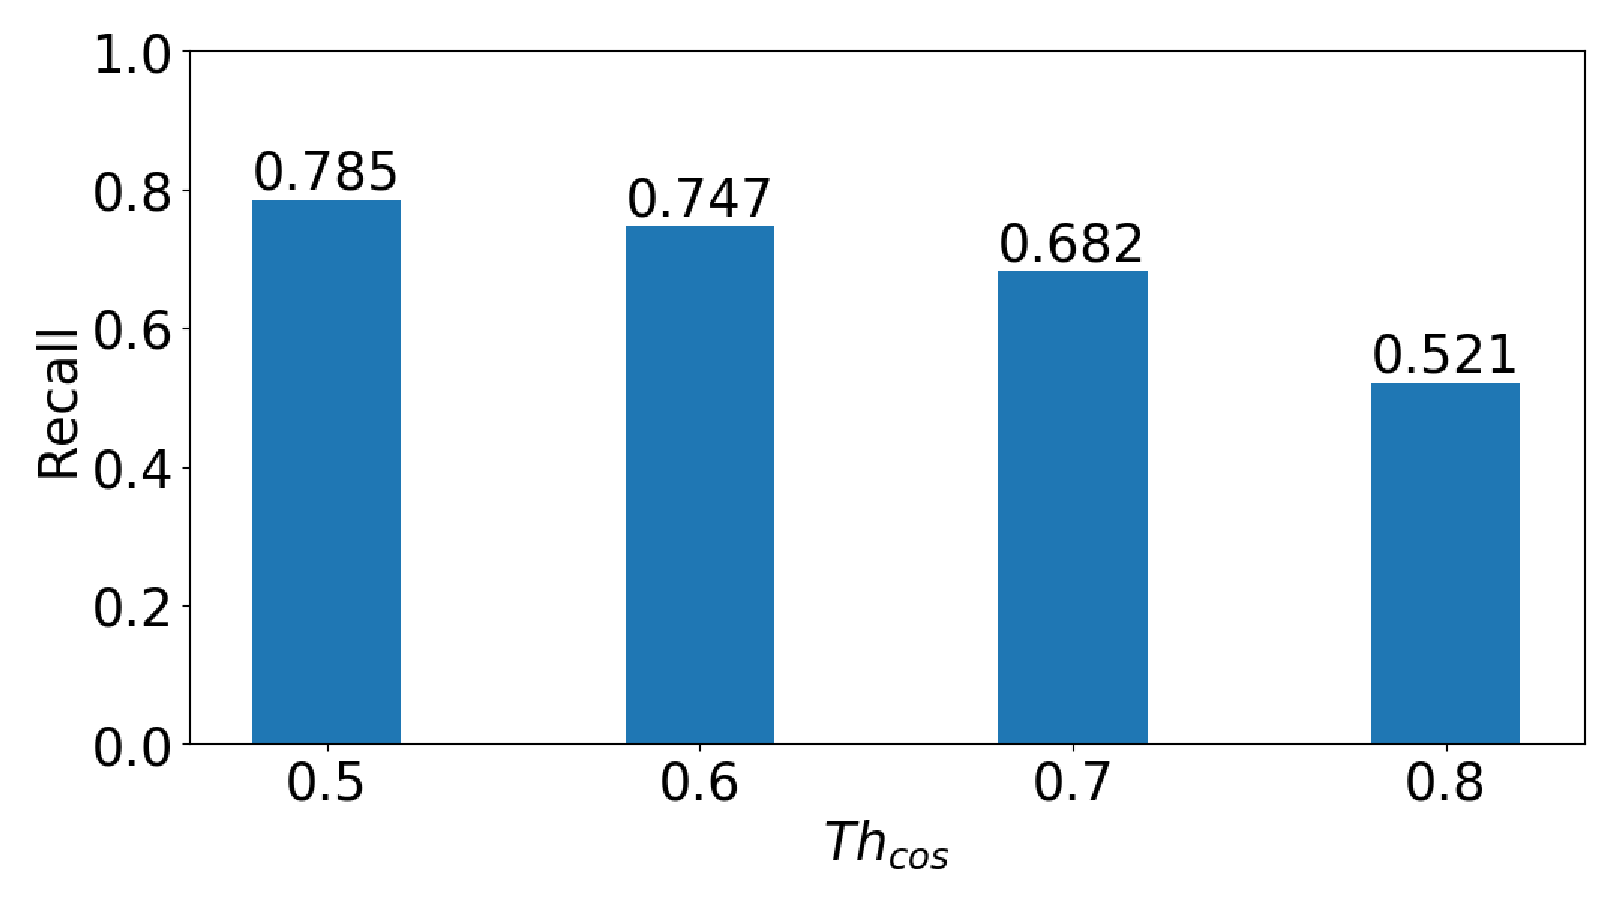
\includegraphics[keepaspectratio, scale=0.25]
                          {./time/figure/prob1_12_r.eps}}
      \end{minipage}

      \begin{minipage}{0.06\hsize}
        \hspace{0.5mm}
      \end{minipage}
 
%----- precision -----
 
      \begin{minipage}{0.40\hsize}
        \centering
          \subfigure[Precision]{\includegraphics[keepaspectratio, scale=0.25]
                          {./time/figure/prob1_12_p.eps}}
      \end{minipage} \\

      \begin{minipage}{0.06\hsize}
        \vspace{5mm}
      \end{minipage} \\
 
 
%----- fmeasure -----
 
      \begin{minipage}{0.40\hsize}
        \centering
          \subfigure[F-measure]{\includegraphics[keepaspectratio, scale=0.25]
                          {./time/figure/prob1_12_f.eps} \label{prob1_fmeasure_time}}
      \end{minipage}

      \begin{minipage}{0.06\hsize}
        \hspace{0.5mm}
      \end{minipage}
 

    
    \end{tabular}
\caption{手法1によるアンカーの発話区間検出精度 ($Th_{time}=1.2$) \label{fig:result_anchor_prob1_time}}
\end{figure} 

\begin{table}[H]
  \begin{center}
    \caption{手法1による各ニュース番組音声のニュースアンカーの発話検出精度($Th_{cos}=0.6,Th_{time}=1.2$) }
    \begin{tabular}{|c||c|c|c|c|} \hline
データID & Recall & Precision & F-meature & 作成したクラスタ数\\ \hline
ニュース1 & 0.989 & 0.779 & 0.872 & 1 \\ \hline
ニュース2 & 0.772 & 0.809 & 0.790 & 2 \\ \hline
ニュース3 & 0.755 & 0.837 & 0.794 & 2 \\ \hline
ニュース4 & 0.637 & 0.732 & 0.681 & 2 \\ \hline
ニュース5 & 0.681 & 0.962 & 0.798 & 2 \\ \hline
計 & 0.748 & 0.823 & 0.784 & - \\ \hline
    \end{tabular}
  \end{center}
\end{table}

%手法2の図
\begin{figure}[H]
  \centering
    \begin{tabular}{c}
 
%----- recall -----
 
      \begin{minipage}{0.40\hsize}
        \centering
          \subfigure[Recall]{\includegraphics[keepaspectratio, scale=0.25]
                          {./time/figure/prob2_r.eps}}
      \end{minipage}

      \begin{minipage}{0.06\hsize}
        \hspace{0.5mm}
      \end{minipage}
 
%----- precision -----
 
      \begin{minipage}{0.40\hsize}
        \centering
          \subfigure[Precision]{\includegraphics[keepaspectratio, scale=0.25]
                          {./time/figure/prob2_p.eps}}
      \end{minipage} \\

      \begin{minipage}{0.06\hsize}
        \vspace{5mm}
      \end{minipage} \\
 
 
%----- fmeasure -----
 
      \begin{minipage}{0.40\hsize}
        \centering
          \subfigure[F-measure]{\includegraphics[keepaspectratio, scale=0.25]
                          {./time/figure/prob2_f.eps} \label{prob2_fmeasure_time}}
      \end{minipage}

      \begin{minipage}{0.06\hsize}
        \hspace{0.5mm}
      \end{minipage}
 
    \end{tabular}
\caption{手法2によるニュースアンカーの発話検出精度 \label{fig:result_anchor_prob2_time}}
\end{figure} 

\begin{table}[H]
  \begin{center}
    \caption{手法2による各ニュース番組音声のニュースアンカーの発話検出精度($Th_{cos}=0.6$) }
    \begin{tabular}{|c||c|c|c|c|} \hline
データID & Recall & Precision & F-meature & 作成したクラスタ数\\ \hline
ニュース1 & 0.981 & 0.689 & 0.810 & 1 \\ \hline
ニュース2 & 0.788 & 0.647 & 0.711 & 2 \\ \hline
ニュース3 & 0.739 & 0.813 & 0.774 & 2 \\ \hline
ニュース4 & 0.644 & 0.736 & 0.687 & 2 \\ \hline
ニュース5 & 0.672 & 0.944 & 0.785 & 2 \\ \hline
計 & 0.745 & 0.761 & 0.753 & - \\ \hline
    \end{tabular}
  \end{center}
\end{table}

%手法3の図
\begin{figure}[H]
  \centering
    \begin{tabular}{c}
 
%----- recall -----
 
      \begin{minipage}{0.40\hsize}
        \centering
          \subfigure[Recall]{\includegraphics[keepaspectratio, scale=0.25]
                          {./time/figure/prob3_11_r.eps}}
      \end{minipage}

      \begin{minipage}{0.06\hsize}
        \hspace{0.5mm}
      \end{minipage}
 
%----- precision -----
 
      \begin{minipage}{0.40\hsize}
        \centering
          \subfigure[Precision]{\includegraphics[keepaspectratio, scale=0.25]
                          {./time/figure/prob3_11_p.eps}}
      \end{minipage} \\

      \begin{minipage}{0.06\hsize}
        \vspace{5mm}
      \end{minipage} \\
 
 
%----- fmeasure -----
 
      \begin{minipage}{0.40\hsize}
        \centering
          \subfigure[F-measure]{\includegraphics[keepaspectratio, scale=0.25]
                          {./time/figure/prob3_11_f.eps} \label{prob3_fmeasure_time}}
      \end{minipage}

      \begin{minipage}{0.06\hsize}
        \hspace{0.5mm}
      \end{minipage}
 
%----- acc time -----
\begin{comment}
      \begin{minipage}{0.40\hsize}
        \centering
          \subfigure[$Acc_{time}$]{\includegraphics[keepaspectratio, scale=0.25]
                          {./figure/prob3_11_acc.eps}}
      \end{minipage}
\end{comment}
    \end{tabular}
\caption{手法3によるアンカーの発話区間検出精度 ($Th_{time}=1.1$) \label{fig:result_anchor_prob3_time}}
\end{figure} 


\begin{table}[H]
  \begin{center}
    \caption{手法3による各ニュース番組音声のニュースアンカーの発話検出精度($Th_{cos}=0.6,Th_{time}=1.1$) \label{table:prob3_eachnews_time}}
    \begin{tabular}{|c||c|c|c|c|} \hline
データID & Recall & Precision & F-meature & 作成したクラスタ数\\ \hline
ニュース1 & 0.988 & 0.780 & 0.872 & 1 \\ \hline
ニュース2 & 0.780 & 0.717 & 0.747 & 2 \\ \hline
ニュース3 & 0.758 & 0.831 & 0.793 & 2 \\ \hline
ニュース4 & 0.623 & 0.758 & 0.684 & 2 \\ \hline
ニュース5 & 0.672 & 0.959 & 0.790 & 2 \\ \hline
計 & 0.744 & 0.808 & 0.775 & - \\ \hline
    \end{tabular}
  \end{center}
\end{table}

実験の結果、各手法とBaseline1を比較したとき、ニュースアンカーの検出精度の指標であるF-measureが手法1では5.9\%(図\ref{prob1_fmeasure_time})、手法2では2.8\%(図\ref{prob2_fmeasure_time})、手法3では5.0\%(図\ref{prob3_fmeasure_time})の向上が確認された。また、各手法とBaseline2を比較したとき、ニュースアンカーの検出精度の指標であるF-measureが手法1では4.8\%、手法2では1.7\%、手法3では3.9\%の向上が確認された。
